\documentclass[11pt, oneside]{article}   	% use "amsart" instead of "article" for AMSLaTeX format
\usepackage{geometry}                		% See geometry.pdf to learn the layout options. There are lots.
\geometry{letterpaper}                   		% ... or a4paper or a5paper or ... 
%\geometry{landscape}                		% Activate for for rotated page geometry
%\usepackage[parfill]{parskip}    		% Activate to begin paragraphs with an empty line rather than an indent
\usepackage{graphicx}				% Use pdf, png, jpg, or eps§ with pdflatex; use eps in DVI mode
								% TeX will automatically convert eps --> pdf in pdflatex		
\usepackage{amssymb}

\usepackage{listings}
\usepackage{color}

\definecolor{dkgreen}{rgb}{0,0.6,0}
\definecolor{gray}{rgb}{0.5,0.5,0.5}
\definecolor{mauve}{rgb}{0.58,0,0.82}

\title{Title Detection System}
\author{Marc Torrellas Socastro}
\date{July 12th, 2019}					% Activate to display a given date or no date

\begin{document}
\maketitle
\section{Abstract}

The package at hand provides a system for Machine Learning (ML) as a service, where the user can train, predict, and evaluate on data describing title candidates in text documents. Sample data for testing, and a model, are also provided, in case the user does not have labelled data to train with. With few data (less than 5k samples), the system achieves high ROC AUC score. Besides, a number of potential future tasks to improve the system in different aspects are proposed.

\section{Problem statement}

The system works with data in a CSV format as follows. Each line represents information about one particular block of text from the document. This information contains:
\begin{itemize}
\item Text: the raw text of the section as interpreted by the OCR;
\item IsBold: is the section bold or not;
\item IsItalic: is the section italic or not;
\item IsUnderlined: is the section underlined or not;
\item Left: the left coordinate on the page;
\item Right: the right coordinate on the page;
\item Top: the top coordinate on the page;
\item Bottom:the bottom coordinate on the page
\item Label: a label to state if the section represents a title (1) or normal text (0). 
\end{itemize}

The objective is to predict, for each sample, whether or not it is a title, i.e. the label, using the rest of features. Notice the difference between Text and the rest of fields, as the former cannot be directly used to feed a ML model, and some numericalisation is required.

\section{Proposed model architecture}

The system provides ML as a service, i.e. the user can train, predict, and evaluate given the data. Fig. \ref{fig:pipelines} describes the high level pipelines associated to each of these 3 functionalities\footnote{Notice we call \textit{detect} to the pipeline associated to predict, to differentiate from the block called \textit{predict}.}. 

\begin{figure}[h!]
\centerline{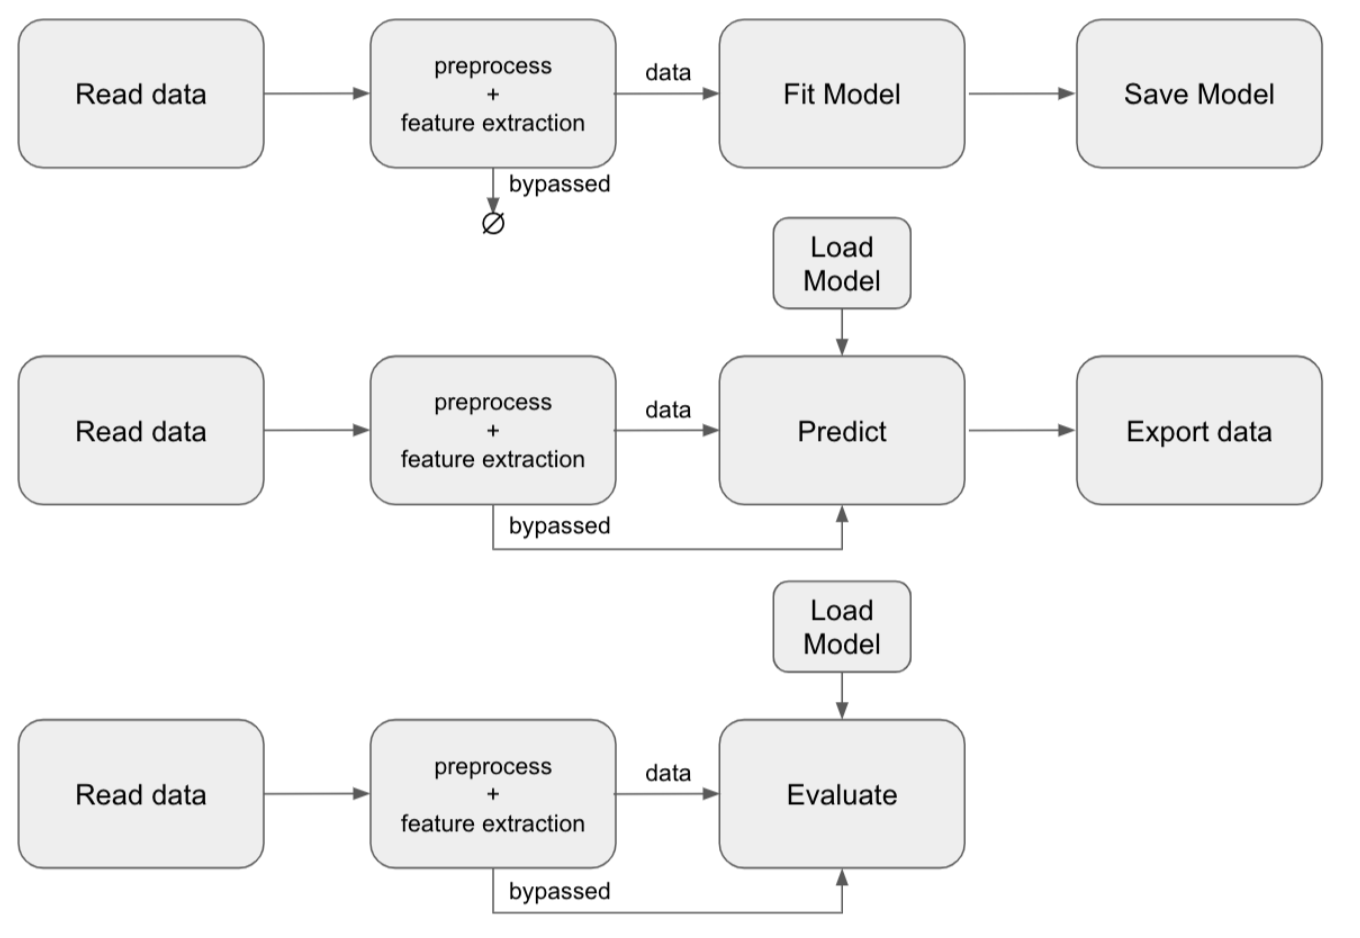
\includegraphics[width=0.8\linewidth]{pipelines.png}} 
\caption{Pipelines for train (top), detect (middle), and evaluate (bottom).}
\label{fig:pipelines}
\end{figure}

Notice that some samples are definitely not titles, e.g. those containing only non-ASCII characters. We found many of those samples in the data, and they are denoted hereafter as \textit{bypassed samples}. 

Given that we have two types of features, we propose to use two models:
\begin{itemize}
\item Slave model: predicts whether the sample is a title or not just by using the text field. We have used a model based on the FastAI library \cite{FastAI}, where first a language model is fine-tuned to the current data, and then the classifier is fit to the task at hand, following the 3-stage ULMFiT methodology \cite{ULMFiT}.
\item Master model: predicts whether the sample is a title or not using all features but the text feature. Here we use not only the fields described in the previous section, but also the output of the slave model, and other spaCy-based features. In this case, we have used a simple feedforward neural network with one hidden layer.
\end{itemize}

\begin{figure}[]
\centerline{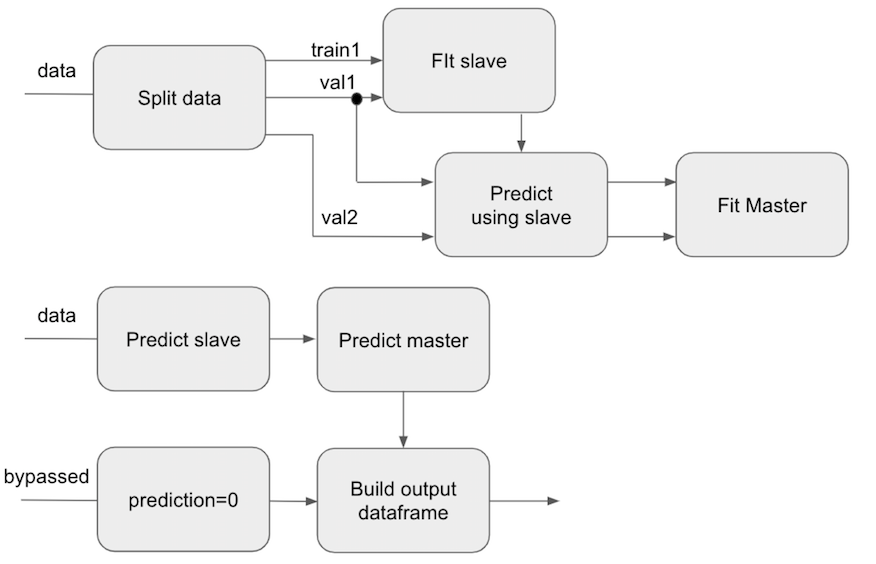
\includegraphics[width=0.8\linewidth]{fit_predict.png}} 
\caption{Pipelines for fit (top), and predict (bottom).}
\label{fig:fit_predict}
\end{figure}

These two models are used in the fit and predict blocks from Fig. \ref{fig:pipelines} as shown in Fig. \ref{fig:fit_predict}. 

\section{Model evaluation}

The proposed architecture has been evaluated for the sample data, both enabling and disabling the slave model.

\subsection{Slave disabled}

In this case, training is really fast, entailing only 8 secs to carry out the train pipeline\footnote{All figures in this report refer to using a MacBook Pro with 4 cores and 8GB RAM}. The results for each dataset in terms of loss and ROC AUC score are detailed next:
\begin{itemize}
\item Train (Loss, Score): 0.1354, 0.9869
\item Val (Loss, Score): 0.1428, 0.9846
\item Test (Loss, Score): 0.1428, 0.9846
\end{itemize}

\subsection{Slave enabled}

In this case, training is really slow, unless we use GPUs. The following durations (using the same machine as above) were recorded:
\begin{itemize}
\item Train the language model: 16 min
\item Train the text classifier: 13 min
\item Predict on validation set 1 with the text classifier: 33 min
\item Predict on validation set 2 with the text classifier: 23 min
\item Train master model: 4 secs
\end{itemize}
while the results for each dataset were:
\begin{itemize}
\item Train (Loss, Score): 0.1106, 0.9906
\item Val (Loss, Score): 0.1216, 0.9882
\item Test (Loss, Score): 0.08549, 0.9954
\end{itemize}

\subsection{Analysis}

Taking into account that we are approaching to the perfect classifier, the improvement from enabling the slave model is significant. However, our recommendation is to enable this mode only in case of having access to GPUs. In our experiments,  the durations above for training and prediction divided by 4.

\section{A brief overview of code architecture}

See \textsf{README.md} for some examples

TODO: did not have time to complete this section


\section{Future work}

While there are many TODOs throughout the code, here we have collected some of the most relevant pending/tentative tasks, and ideas for the following version.

\subsection{Model: performance}

\begin{itemize}
\item Optimise master and slave jointly. At the moment, the optimisation of slave does not take into account that there is a master model taking its predictions as inputs.
\item Analyse the data to see if there are more candidate patterns to be bypassed
\item Using spaCy large model might help, as it contains a better tokeniser
\item Augment feature space using more spaCy based features: NER counts, PoS counts, LDA...
\item Use soft predictions (the score rather than a binary output) from the slave model. If so, it is fundamental to calibrate scores \cite{calibration}.
\item Tune hyper-parameters and use early stopping. Use nested cross-validation (CV) if not a lot of data, to avoid too optimistic performance estimations.
\item In a real situation, given this data we would use all data to train after having measured performance with test
\item The problem can be transformed to sequence tagging if the document each sample belongs to was provided. There are many popular architectures for this, e.g:
\begin{itemize}
     \item Use handcrafted features and a Conditional Random Field (CRF)\cite{CRF}
     \item Use the popular BiLSTM + CRF architecture \cite{BiLSTM_CRF}
     \item Use a Transformer\cite{Transformer}-based architecture like BERT \cite{BERT}
   \end{itemize}
\item Experiment using newer stuff like BERT, GPT, XLnet
\end{itemize}

\subsection{Model: usability}

\begin{itemize}
\item Allow the user to get soft scores from command-line arguments.
\item Columns are changing names in the output dataframe. This might be an issue for some users. If so, it's not difficult to keep the original names.
\item If the code is too slow, a non deep learning solution (with the data provided, at least) provides similar performance and probably faster, see notebooks.
\item Turn the config file to raw text file, and allow the user to pass a config file to use alternative settings
\item Fix all random seeds for the sake of reproducibility. Clients expect to see same results after carrying out same operations with same data
\end{itemize}

\subsection{Model: evaluation}

\begin{itemize}
\item Use cross-validation to get a more accurate evaluation of performance, together with a measure of confidence for the score
\item Use other scorers, e.g. F-score given that data is imbalanced, or even better, F-score gain \cite{PRG}.
\item The loss when \textit{evaluate} is not considering the bypassed. Probably it would not change dramatically, but the figures are not rigorously correct.
\end{itemize}

\subsection{Coding: readability}

\begin{itemize}
\item Some of the lines in \textsf{pipelines.py} are very similar, or even duplicated. Structuring the code in a better way would allow (a) to improve readability, and (b) to update all occurrences more efficiently.
\item Add more docstrings and review naming
\end{itemize}

\subsection{Coding: efficiency}

\begin{itemize}
\item Because the lack of time, we did not have time to investigate how to predict more efficiently using the fastAI model. Hence, we implemented a for loop and predicted sample by sample. We proposed in the TODOs a way to parallelise using \textsf{concurrent.futures}, but didn't have time to test everything again. With some small experiments, it seems to divide by about the number of cores the prediction time. This is however not a problem in case of having GPUs, see experiments in notebook using Google Colab.
\item It does not seem necessary to save the two fastAI-based models (language model and classifier) to disk.
\end{itemize}

\subsection{Coding: others}

\begin{itemize}
\item Write tests to reduce the cost of deployment, and releasing new versions
\item Because the lack of familiarity with packaging and setuptools (it's the first time used), we did not manage to find a way to default to sample data without being in the project folder. We suspect a \textsf{MANIFEST.ini} is required, but didn't have time to finish this.
\item \textsf{setup.py} is a bit hacky right now, calling ``\textsf{python -m spacy download en\_core\_web\_sm}". We opt for this because we did not find a way to install the spaCy language model using \textsf{setuptools}.
\item Use \textsf{Fire} rather than argparse

\end{itemize}

\subsection{Report}

\begin{itemize}
\item Explain more in detail what features are used.
\item Explain the different hyper-parameters used, e.g. batch size, epochs, etc
\item Explain the architecture of slave and master models more in detail.
\item Explain the code architecture, and user interface
\item Present the results in a more compact and visual way, and more results, e.g. confusion matrices.
\item Cite the published papers, not the ArXiv ones, when available.
\end{itemize}

%\bibliographystyle{IEEEbib}
\bibliographystyle{ieeetr}
\bibliography{refs}

\end{document}  